\documentclass{beamer}
\usefonttheme[onlymath]{serif}
\usetheme{Frankfurt}
%\setbeamercovered{transparent}
%\beamertemplatenavigationsymbolsempty

\usepackage[ngerman]{babel}
\usepackage[utf8]{inputenc}
%\usepackage[ansinew]{inputenc}
\usepackage{lmodern}
\usepackage[T1]{fontenc}
\usepackage{amsmath}
\usepackage{amsfonts}
\usepackage{amssymb}
\usepackage{graphicx}
\usepackage{nicefrac}
\usepackage{enumitem}
\usepackage{color}
\usepackage{listings}
\usepackage{color}
%\usepackage{beamerthemeshadow}
\usepackage{autonum}
%\usepackage[style=numeric]{biblatex}
\usepackage{verbatim}
%\usepackage{romanbar}
\usepackage{tikz,pgfplots}
\usetikzlibrary{shapes.misc}
\usetikzlibrary{matrix}

\setbeamertemplate{enumerate items}{enumerate item,enumerate subitem,enumerate subsubitem,enumerate mini template}{}

\setbeamertemplate{headline}
{
  \leavevmode%
  \hbox{%
  \begin{beamercolorbox}[wd=0.5\paperwidth,ht=2.25ex,dp=1ex,center]{section in head/foot}%
    \usebeamerfont{section in head/foot}\insertsection
  \end{beamercolorbox}%
  \begin{beamercolorbox}[wd=0.5\paperwidth,ht=2.25ex,dp=1ex,center]{author in head/foot}%
      \usebeamerfont{subsection in head/foot}\insertsubsection
    \end{beamercolorbox}%
  }%
  \vskip0pt%
}
\setbeamertemplate{footline}
{
  \leavevmode%
  \hbox{%
  \begin{beamercolorbox}[wd=.5\paperwidth,ht=2.25ex,dp=1ex,center]{title in head/foot}%
    \usebeamerfont{author in head/foot}\insertshortauthor
  \end{beamercolorbox}%
  \begin{beamercolorbox}[wd=.5\paperwidth,ht=2.25ex,dp=1ex,center]{author in head/foot}%
    \usebeamerfont{title in head/foot}\insertshorttitle\hspace*{3em}
    \insertframenumber{} / \inserttotalframenumber\hspace*{1ex}
  \end{beamercolorbox}}%
  \vskip0pt%
}

\setbeamertemplate{navigation symbols}{}
\setbeamertemplate{bibliography item}{[\theenumiv]}

\title[Bayesian Inference]{Bayesian Inference}
\subtitle{Seminar - Optimierung in Machine Learning}
\author{Daniel Luft, Fabian Gernandt}
\date{\today}

%\graphicspath{/media/fabian/USB_STICK/Master/2. Semester/Seminar/Grafiken}

\begin{document}
{
\frame{\titlepage}
\frame{
	\frametitle{Inhaltsverzeichnis}
	\tableofcontents
}
\newcommand{\labelitemi}{$\bullet$}
\newcommand{\labelitemii}{$\rightarrow$}

\section{Mathematische Grundlagen}

\frame{\tableofcontents[currentsection,subsectionstyle=show/shaded,hideothersubsections]}

\subsection{Grundlagen der Bayes Statistik}

%Ziele klar benennen: Statistischer Zugang; Grundbegriffe kennen; Idee/ Konzept: Verteilungsannahme --> Probleme; punktuelles Wissen über Verfahren

\begin{frame}{Motivation}
	\begin{itemize}
		\item Was ist und wozu braucht man Bayes Theorie ?
		\begin{itemize}
			\pause \item Grundlage der Lerntheorie
			\pause \item Erzeugung von mathematischen Problemen basierend auf Verteilungsannahmen
			\pause \item Basis für Modellselektion
			\pause \item Kombination von Modellannahmen und Daten
		\end{itemize}
	\end{itemize}
	% Frequentist vs Bayesianer Diagramm
\end{frame}

%eigentlich wäre hier ein Diagramm geiler

\begin{frame}
Möchten ein Modell erstellen, welches Beziehung zwischen Objekten beschreibt.

\begin{itemize}
\item Was sind und wie wählen wir die Parameter $\theta \in \mathbb{R}^n$ des Modells?
\item Berücksichtigen wir die Art wie Samples generiert werden?
\item Wie vergleichen wir mehrere Modelle?
\item Wie passen wir Hyperparameter an?
\end{itemize}
 
  
% MOTIVATION MIT KREUZVALIDIERUNG UND WIE MAN SAMPLET!!
\end{frame}

\begin{frame}
\centering
	\begin{tikzpicture}
		\tikzstyle{sum} = [draw, circle, minimum size=0.8cm, node distance=1.75cm]
		\tikzstyle{block} = [draw, rectangle, minimum width = 2cm, minimum height = 0.5cm]
		
		\onslide<1->{\node [block, minimum width=1cm] (y) at (2,-2.5) {Output};
		\node [block, minimum width=1cm] (X) at (0,0) {Input}; 
		\node [block] (w) at (5,0) {Parameter};
		\node[block, fill=white] (M) at (2, 0) {Modell};
		\draw[->,thick] (w) -- (M);
		\draw[->,thick] (X) -- (M);
		\draw[->,thick] (M) -- (y);}

		\onslide<2->{\node[red,block, minimum width=1cm] (eps) at (5, -1.8) {Fehlerverteilung};
		\draw[red,->,thick] (eps) -- (2.01, -1.8);}

		\onslide<3->{\draw[red,->,thick] (eps) -- (w) node[fill=white, midway, minimum width=1cm] {beeinflusst Wahl};}

		\onslide<4->{\node[block, fill=white] (p) at (5, 1.5) {?};
		\draw[->,thick] (p) -- (w);}
	\end{tikzpicture}
\end{frame}

\begin{frame}
	\centering
	\begin{tikzpicture}
		\tikzstyle{sum} = [draw, circle, minimum size=0.8cm, node distance=1.75cm]
		\tikzstyle{block} = [draw, rectangle, minimum width = 2.75cm, minimum height = 0.5cm]
		
		\onslide<1->{\node [sum] (y) at (2,-3) {$y$};
		\node [sum] (eps) at (0,0) {$\varepsilon$}; 
		\node [sum] (X) at (2,0) {$X$}; 
		\node [sum] (w) at (4,0) {$w$};
		\node [block, fill=white] (M) at (2, -1.5) {$y = Xw+\varepsilon$};
		\draw[->,thick] (eps) -- (M);
		\draw[->,thick] (w) -- (M);
		\draw[->,thick] (X) -- (M);
		\draw[->,thick] (M) -- (y);}
		
		\onslide<2->{\node [sum, red] (lambda) at (0,2) {$\sigma$};
		\draw[->,thick, red] (lambda) -- (eps) node[block,minimum width=1cm, midway, fill=white] {$\varepsilon\sim N(0,\sigma^2 I_n)$};}
	\end{tikzpicture}
	%HIER KURZ AUF REGRESSION KOMMEN! UND DAMIT ML SCHÄTZER MOTIVIEREN + UNTERSCHIED ZWISCHEN VERSCHIEDENEN PARAMETERN
\end{frame}

%R package nnet benutzt ML schätzer um weights bei neural networks zu bestimmen!!!! hat aber nachteile, z.b. schwer zu optimierende probleme mit sattelpunkten je nachdem

\begin{frame}{ML-Schätzer}
% NOTATION ERKLÄREN

Sei $X=(x_1,...,x_n)$ ein i.i.d. Datenvektor der modellierten Zufallsvariable $X$ mit Verteilungsparameter $\theta\in\mathbb{R}^n$. Dann definieren wir die Likelihoodfunktion durch

\begin{center}
$\mathcal{L}( \theta \vert x):= \mathbb{P}(x_1,...,x_n\vert \theta) =\overset{n}{\underset{i=1}{\prod}}\mathbb{P}(x_i\vert \theta).$
\end{center}
 Weiterhin heißt
\begin{center}
$\hat{\theta}_{ML} := \arg\underset{\theta \in \Theta}{\max} \mathcal{L}( \theta \vert x)$
\end{center}

Maximum-Likelihood-Schätzer von $\theta$.

\end{frame}


%hier vielleicht sofort mit latenten Variablen kommen! und erklären + proportionalität als wichtige relation (normfaktor oft unwichtig bei opt!)

\begin{frame}
\begin{block}{Definition: A priori Verteilung}
Seien die Modellparameter $\theta$ eine $\mathbb{R}^n$-wertige Zufallsvariable. Dann heißt ihre Verteilung $\mathbb{P}(\theta)$ a priori Verteilung.

\end{block}


\end{frame}


\begin{frame}{Beispiel: Münzwurf}

	\begin{minipage}{7cm}
		Modelliere einen Münzwurf $X$! Annahmen:
		
		Modell:
		
		$X \sim Ber(p)$ mit Werten Kopf und Zahl.
		
		Prior:
		
		$p \sim Beta(\alpha,\beta)$\\
		\begin{align}
			f_{Beta}\left(x\vert\alpha,\beta\right)\;=\;\dfrac{\varGamma(\alpha+\beta)}{\varGamma(\alpha)\varGamma(\beta)}\;x^{\alpha-1}(1-x)^{\beta-1}
		\end{align}
	\end{minipage}
	\begin{minipage}{3cm}
		\flushright
		\pause
		\begin{tikzpicture}
			\tikzstyle{sum} = [draw, circle, minimum size=0.8cm, node distance=1.75cm]
			\tikzstyle{block} = [draw, rectangle, minimum width = 2.75cm, minimum height = 0.5cm]
			
			\onslide<1->{\node [sum] (y) at (2,-2.5) {$y$};
			\node [sum] (X) at (2,0) {$X$}; 
			\node [sum] (p) at (2,2) {$p$};
			\node [block, fill=white, minimum width = 2cm] (M) at (2, -1.25) {$y = 2X$};
			\draw[->,thick] (X) -- (M);
			\draw[->,thick] (M) -- (y);
			\draw[->,thick] (p) -- (X) node[block, fill=white, midway, minimum width=1cm] {$X\sim Ber(p)$};}

			\pause
			\onslide<2->{\node [block, red] (Beta) at (2, 3.25) {$p\sim Beta(\alpha, \beta)$};
			\node [sum,red] (alpha) at (1,4.5) {$\alpha$};
			\node [sum,red] (beta) at (3,4.5) {$\beta$};
			\draw[->,thick,red] (alpha) -- (Beta);
			\draw[->,thick,red] (beta) -- (Beta);
			\draw[->,thick,red] (Beta) -- (p);}
		\end{tikzpicture}
	\end{minipage}
\end{frame}



%überleitung mit welche parameterverteilung ist wohl gut + was dann
%und was wenn x nicht iid? --> dann muss man marginalverteilung hochdimensional berechnen... also kacke --> führt auch zu EM und VBayes

\begin{frame}
	\begin{block}{Satz von Bayes (Bayes 1763, Laplace 1812)}
		Sei $(\Omega, \mathcal{A}, \mathbb{P})$ ein Wahrscheinlichkeitsraum. Seien $A,B \in \mathcal{A}$ Ereignisse. Dann gilt:
		\begin{center}
			$\mathbb{P}(A\vert B) = \frac{\mathbb{P}(B \vert A) \mathbb{P}(A)}{\mathbb{P}(B)}$
		\end{center}
	\end{block}
\end{frame}

\begin{frame}{Trainieren des Priors: Posterior}
	\begin{block}{Definition: A posteriori Verteilung}
	Seien $\theta$ Modellparameter des Modells mit a priori Verteilung $\mathbb{P}(\theta)$. Sei $x=(x_1,...,x_n)$ ein Datenvektor aus Realisationen von $X$. Dann heißt
	\begin{center}
		$\mathbb{P}(\theta\vert x):= \frac{\mathbb{P}(x\vert \theta)\mathbb{P}(\theta)}{\mathbb{P}(x)}=
		\frac{\mathbb{P}(x\vert \theta)\mathbb{P}(\theta)}{\int\mathbb{P}(x\vert \theta)d\mathbb{P}(\theta)}$
	\end{center}
	die a posteriori Verteilung von $\theta$.
	\end{block}
\end{frame}


\begin{frame}{Traditioneller Bayesianischer Ansatz:}

Behandle Parameter $\theta$ wie Zufallsvariablen mit Verteilung $\mathbb{P}(\theta \vert x)$:\\
\begin{itemize}
	\pause \item berechne Momente (Erwartungswert, Varianz...)
	\pause \item berechne Konfidenzintervalle
	\pause \item berechne Quantile
	\pause \item ...
\end{itemize}
\pause Beispiel:
\begin{center}
$\hat{\theta}_{Bayes} = \mathbb{E}_{\theta \vert x}[\theta]$
\end{center}

%ACHTUNG: POSTERIOR KOMPLETT BERECHNEN --> NEUE PROBLEME UND ALGORITHMEN

\end{frame}


%cross validation erwähnen

\begin{frame}
\begin{block}{Definition: MAP Schätzer}

Sei $x= (x_1,\dots,x_n)$ ein Datenvektor generiert durch $X$. Weiterhin sei $\mathbb{P}(\theta)$ die a priori Verteilung der Parameter $\theta$. Dann heißt

\begin{align}
\hat{\theta}_{MAP} & := \arg\underset{\theta \in \Theta}{\max}\hspace{0.3mm} \mathbb{P}(\theta \vert x)
\end{align}


Maximum a posteriori-Schätzer für $\theta$.
\end{block}
\end{frame}

%bsp münzwurf mit gezinkter Münze?

\begin{frame}

Es gelten die folgenden Transformationen des MAP-Schätzers:

\begin{align}
\hat{\theta}_{MAP} & := \arg\underset{\theta \in \Theta}{\max}\hspace{0.3mm} \mathbb{P}(\theta \vert x) \\ & =  
 \arg\underset{\theta \in \Theta}{\max} \frac{ \mathbb{P}(x\vert\theta) \mathbb{P}(\theta)}{\int  \mathbb{P}(x\vert \theta) d\mathbb{P}(\theta)}\\
 & = \arg\underset{\theta \in \Theta}{\max}  \mathbb{P}(x\vert \theta) \mathbb{P}(\theta) \\
 & = \arg\underset{\theta \in \Theta}{\max} \log\mathbb{P}(x\vert \theta) + \log \mathbb{P}(\theta)
\end{align}

\end{frame}

\subsection{Einführendes Beispiel}



\section{Bayesian Regression}

\frame{\tableofcontents[currentsection,subsectionstyle=show/shaded,hideothersubsections]}

\subsection{Ridge-Regression}

% Ridge aus numerischer Richtung "herleiten" -> Eigenwerte, Konditionierung, Levenberg-Marquardt, Multikollinearität
% https://stats.stackexchange.com/questions/151304/why-is-ridge-regression-called-ridge-why-is-it-needed-and-what-happens-when

\begin{frame}{Regressionsmodell}
	\centering
	\begin{tikzpicture}
		\tikzstyle{sum} = [draw, circle, minimum size=0.8cm, node distance=1.75cm]
		\tikzstyle{block} = [draw, rectangle, minimum width = 2.75cm, minimum height = 0.5cm]
		\node [sum] (y) at (2,-3) {$y$};
		\node [sum] (eps) at (0,0) {$\varepsilon$}; 
		\node [sum] (X) at (2,0) {$X$}; 
		\node [sum] (w) at (4,0) {$w$};
		\node [block, fill=white] (M) at (2, -1.5) {$y = Xw+\varepsilon$};
		\node [sum, red] (lambda) at (0,2) {$\sigma$};
		%\node [red, sum] (alpha) at (4,2) {$\alpha$};

		\draw[->,thick] (eps) -- (M);
		\draw[->,thick] (w) -- (M);
		\draw[->,thick] (X) -- (M);
		\draw[->,thick] (M) -- (y);
		%\draw[->,thick] (X) -- (y) node[block, midway, fill=white] {$y = Xw+\varepsilon$};
		\draw[->,thick, red] (lambda) -- (eps) node[block,minimum width=1cm, midway, fill=white] {$\varepsilon\sim \mathcal{N}(0,\sigma^2 I_n)$};
		%\draw[red,->,thick] (alpha) -- (w) node[block,minimum width=1cm, midway, fill=white] {$w\sim N(0,\alpha I_k)$}; 
	\end{tikzpicture}
\end{frame}

\begin{frame}{Wiederholung OLS-Schätzer}
	Zielfunktional der multiplen linearen Regression:
	\begin{align}
		\hat{w}&\;=\;\arg\underset{w}{\min}\left[\left(y-\hat{y}\right)^T\left(y-\hat{y}\right)\right] \\
		&\;=\;\arg\underset{w}{\min}\left[\left(y-Xw\right)^T\left(y-Xw\right)\right]\\
	\end{align}\pause
	Der (analytische) Schätzer für $w$ ergibt sich durch:
	\begin{align}
		\hat{w}\;=\;\left(X^TX\right)^{-1}Xy
	\end{align}\pause
	$\rightarrow\: X^TX$ zwar immer positiv semidefinit, kann aber schlecht konditioniert sein
\end{frame}

\begin{frame}{Ridge-Schätzer}
	Idee: Verwende anderen Schätzer, welcher besser konditioniert ist.
	\begin{itemize}\pause
		\item[$\rightarrow$] Ridge-Schätzer, nach Tikhonov/Tychonoff (1963)
	\end{itemize}
	\begin{align}
		\hat{w}_{Ridge}\;=\;\left(X^TX+\lambda I\right)^{-1}Xy
	\end{align}\pause
	\begin{itemize}
		\item[$\rightarrow$] Ridge-Schätzer schon für kleines $\lambda$ gut konditioniert
		\item[$\rightarrow$] Varianzen sind geringer, als beim OLS-Schätzer
		\item[$\rightarrow$] Aber: der Schätzer ist verzerrt
	\end{itemize}
\end{frame}

\begin{frame}{Ridge-Regression}
	Der Ridge-Schätzer minimiert folgendes Zielfunktional:
	\begin{align}
		\hat{w}_{Ridge}\;=\;\arg\underset{w}{\min}\left[\left(y-Xw\right)^T\left(y-Xw\right)+\lambda w^Tw\right]
	\end{align}\pause
	\hfill\\[0,5cm]
	Es soll nun das obige Funktional mit Bayes Ansatz hergeleitet werden. Die grundlegenden Annahmen der linearen Regression können zunächst wie folgt interpretiert werden:
	\begin{align}
		\mathbb{P}(y_i\vert w)\;=\;\mathcal{N}(X_iw,\sigma^2)
	\end{align}
\end{frame}

\begin{frame}{Regressionsmodell}
	\centering
	\begin{tikzpicture}
		\tikzstyle{sum} = [draw, circle, minimum size=0.8cm, node distance=1.75cm]
		\tikzstyle{block} = [draw, rectangle, minimum width = 2.75cm, minimum height = 0.5cm]
		\node [sum] (y) at (2,-3) {$y$};
		\node [sum] (eps) at (0,0) {$\varepsilon$}; 
		\node [sum] (X) at (2,0) {$X$}; 
		\node [sum] (w) at (4,0) {$w$};
		\node [block, fill=white] (M) at (2, -1.5) {$y = Xw+\varepsilon$};
		\node [sum] (lambda) at (0,2) {$\sigma$};

		\draw[->,thick] (eps) -- (M);
		\draw[->,thick] (w) -- (M);
		\draw[->,thick] (X) -- (M);
		\draw[->,thick] (M) -- (y);
		\draw[->,thick] (lambda) -- (eps) node[block,minimum width=1cm, midway, fill=white] {$\varepsilon\sim \mathcal{N}(0,\sigma^2 I_n)$};
		\onslide<2->{\node [red, sum] (alpha) at (4,2) {$\tau$};
		\draw[red,->,thick] (alpha) -- (w) node[block,minimum width=1cm, midway, fill=white] {$w\sim \mathcal{N}(0,\tau^2 I_k)$};}
	\end{tikzpicture}
\end{frame}

\begin{frame}{Bayesian-Ridge}
	A priori Annahmen für Fehler $\varepsilon$ und Gewichte $w$ bei der Bayesian-Ridge-Regression:
	\begin{align}
		\varepsilon\sim \mathcal{N}(0, \sigma^2 I_n),\quad w\sim \mathcal{N}(0, \tau^2 I_k)
	\end{align}\pause
	Mit der Likelihood und den a priori Annahmen folgt:
	\begin{align}
		\mathcal{L}(w|y)&\;=\;\mathbb{P}(y|w)\\
		&\;=\;\prod_{i=1}^{n}\mathbb{P}(y_i|w)\\
		&\;=\;\prod_{i=1}^{n}\frac{1}{\sigma\sqrt{2\pi}}\exp\left(-\frac{\left(y_i-X_iw\right)^2}{2\sigma^2}\right)
	\end{align}
\end{frame}

\begin{frame}{Bayesian-Ridge}
	Mit der Transformation des Maximum a posteriori-Schätzers ergibt sich:
	\begin{alignat}{2}
		\hat{w}_{\text{MAP}}&\;=\;\arg\underset{w}{\max}&& \log\mathbb{P}(y\vert w) + \log \mathbb{P}(w) \\
		\uncover<2->{&\;=\;\arg\underset{w}{\max}&&\left[\log\left(\prod_{i=1}^{n}\frac{1}{\sigma\sqrt{2\pi}}\exp\left(-\frac{\left(y_i-X_iw\right)^2}{2\sigma^2}\right)\right)\right.\\	&\hspace{1,7cm}+&&\:\:\left.\log\left(\prod_{i=1}^{k}\frac{1}{\tau\sqrt{2\pi}}\exp\left(-\frac{w_i^2}{2\tau^2}\right)\right)\right]}\\
		\uncover<3->{&\;=\;\arg\underset{w}{\max} && \left[-\sum_{i=1}^{n}\frac{\left(y_i-X_iw\right)^2}{2\sigma^2}-\sum_{i=1}^{k}\frac{w_i^2}{2\tau^2}\right]}\\
	\end{alignat}
\end{frame}

\begin{frame}{Bayesian-Ridge}
	\begin{alignat}{2}
		&\;=\;\arg\underset{w}{\max} && \left[\frac{1}{2\sigma^2}\left(-\sum_{i=1}^{n}\left(y_i-X_iw\right)^2-\frac{\sigma^2}{\tau^2}\sum_{i=1}^{k}w_i^2\right)\right]\\
		\uncover<2->{&\;=\;\arg\underset{w}{\min} && \left[\sum_{i=1}^{n}\left(y_i-X_iw\right)^2+\lambda\sum_{i=1}^{k}w_i^2\right]} \\
	\end{alignat}\pause\pause
	Damit erhält man das Ridge-Optimierungsproblem
	\begin{align}
		\hat{w}_{MAP}\;=\;\arg\underset{w}{\min}\left[\left(y-Xw\right)^T\left(y-Xw\right)+\lambda w^Tw\right]
	\end{align}
\end{frame}

\subsection{Lasso-Regression}

\begin{frame}{Bayesian-Lasso}
	Neue Annahme: $w\sim Laplace(0, \tau)$ mit der Dichte
	\begin{align}
		f_{Laplace}(x|\mu,\tau)\;=\;\frac{1}{2\tau}\exp\left(-\frac{\left|x-\mu\right|}{\tau}\right)
	\end{align}\pause
	\centering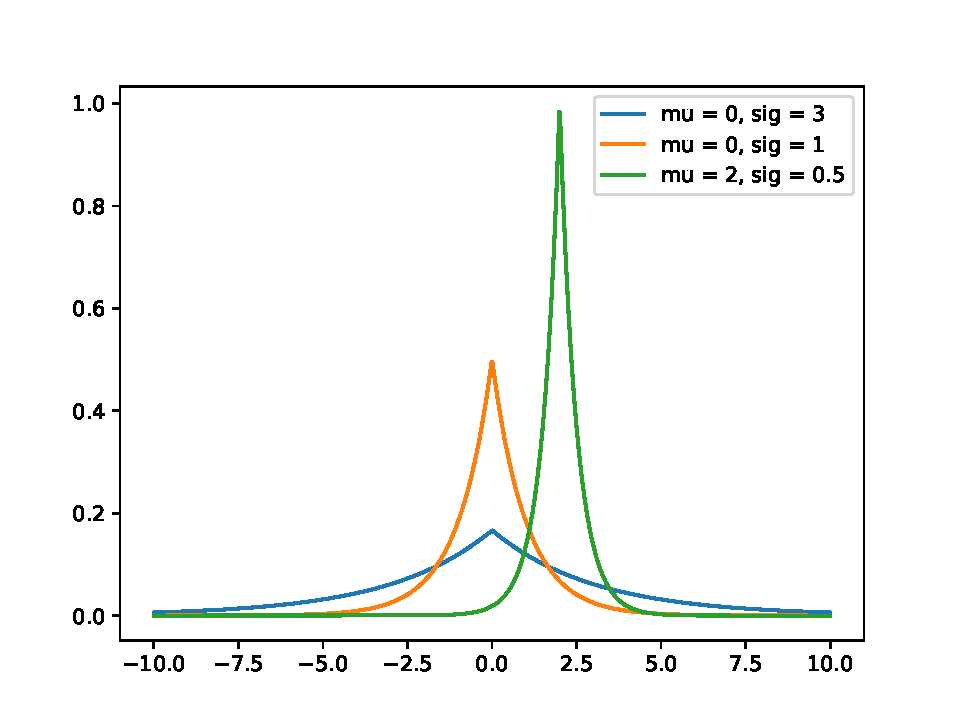
\includegraphics[scale=0.45]{laplacedens.pdf}
\end{frame}

\begin{frame}{Regressionsmodell}
	\centering
	\begin{tikzpicture}
		\tikzstyle{sum} = [draw, circle, minimum size=0.8cm, node distance=1.75cm]
		\tikzstyle{block} = [draw, rectangle, minimum width = 2.75cm, minimum height = 0.5cm]
		\node [sum] (y) at (2,-3) {$y$};
		\node [sum] (eps) at (0,0) {$\varepsilon$}; 
		\node [sum] (X) at (2,0) {$X$}; 
		\node [sum] (w) at (4,0) {$w$};
		\node [block, fill=white] (M) at (2, -1.5) {$y = Xw+\varepsilon$};
		\node [sum] (lambda) at (0,2) {$\sigma$};
		\node [red, sum] (alpha) at (4,2) {$\tau$};

		\draw[->,thick] (eps) -- (M);
		\draw[->,thick] (w) -- (M);
		\draw[->,thick] (X) -- (M);
		\draw[->,thick] (M) -- (y);
		\draw[->,thick] (lambda) -- (eps) node[block,minimum width=1cm, midway, fill=white] {$\varepsilon\sim \mathcal{N}(0,\sigma^2 I_n)$};
		\draw[red,->,thick] (alpha) -- (w) node[block,minimum width=1cm, midway, fill=white] {$w\sim \mathcal{N}(0,\tau^2 I_k)$};
		\onslide<2->{\draw[red,->,thick] (alpha) -- (w) node[block,minimum width=1cm, midway, fill=white, minimum height=0.7cm] {$w\sim Laplace(0,\tau I_k)$};}
	\end{tikzpicture}
\end{frame}

\begin{frame}{Bayesian-Lasso}
	Mit der Annahme der laplaceverteilten Parameter folgt:
	\begin{alignat}{2}
		\hat{w}_{\text{MAP}}&\;=\;\arg\underset{w}{\max}&& \log\mathbb{P}(y\vert w) + \log \mathbb{P}(w) \\
		\uncover<2->{&\;=\;\arg\underset{w}{\max}&&\left[\log\left(\prod_{i=1}^{n}\frac{1}{\sigma\sqrt{2\pi}}\exp\left(-\frac{\left(y_i-X_iw\right)^2}{2\sigma^2}\right)\right)\right.\\	&\hspace{1,7cm}+&&\:\:\left.\log\left(\prod_{i=1}^{k}\frac{1}{2\tau}\exp\left(-\frac{\left|w_i\right|}{\tau}\right)\right)\right]}\\
		\uncover<3->{&\;=\;\arg\underset{w}{\max} && \left[-\sum_{i=1}^{n}\frac{\left(y_i-X_iw\right)^2}{2\sigma^2}-\sum_{i=1}^{k}\frac{\left|w_i\right|}{\tau}\right]}\\
	\end{alignat}
\end{frame}

\begin{frame}{Bayesian-Lasso}
	\begin{alignat}{2}
		&\;=\;\arg\underset{w}{\max} && \left[\frac{1}{2\sigma^2}\left(-\sum_{i=1}^{n}\left(y_i-X_iw\right)^2-\frac{\sigma^2}{2\tau}\sum_{i=1}^{k}\left|w_i\right|\right)\right]\\
		\uncover<2->{&\;=\;\arg\underset{w}{\min} && \left[\sum_{i=1}^{n}\left(y_i-X_iw\right)^2+\lambda\sum_{i=1}^{k}\left|w_i\right|\right]} \\
	\end{alignat}\pause\pause
	Damit erhält man das Lasso-Optimierungsproblem
	\begin{align}
		\hat{w}_{MAP}\;=\;\arg\underset{w}{\min}\left[\left(y-Xw\right)^T\left(y-Xw\right)+\lambda\sum_{i=1}^{k}\left|w_i\right|\right]
	\end{align}\pause
	$\rightarrow\:$ least absolute shrinkage and selection operator
\end{frame}

\section{Bayesian Framework für SVM}

\frame{\tableofcontents[currentsection,subsectionstyle=show/shaded,hideothersubsections]}

\subsection{Wiederholung SVM}
%support vector machines beispiel mit ovarian tumors

\begin{frame}{Wiederholung: klassische Support Vector Machine}
Gegeben ist ein Datensatz $(x_i,y_i)_{i=1,...,n}$ von Features $x_i$ und Klassen $y_i = \pm 1$.

%WAS SIND DIE RICHTIGEN ANNAHMEN GEWESEN?

\pause
\begin{block}{Primales Problem}
	\begin{center}
	$ \underset{w, b}{\min} \frac{1}{2}\vert \vert w \vert \vert ^2_2$\\
	unter $ y_i(w^T x_i + b) \geq 1$
	\end{center}
\end{block}

\pause
\begin{block}{Duales Problem}
	\begin{center}
	$\underset{\lambda}{\min} \frac{1}{2}\underset{i,j}{\sum} \lambda_i \lambda_j y_i y_j x_i^T x_j - \underset{i}{\sum}\lambda_i$ \\
	unter $\underset{i}{\sum}\lambda_i y_i = 0, 0 \leq \lambda_i $
	\end{center}
\end{block}

\end{frame}

\begin{frame}{Wiederholung: Support Vector Machine mit Soft Margin}

Gegeben ist ein Datensatz $(x_i,y_i)_{i=1,...,n}$ von Features $x_i$ und Klassen $y_i = \pm 1$.

\pause
\begin{block}{Primales Problem}
	\begin{center}
	$ \underset{w, b}{\min} \frac{1}{2}\vert \vert w \vert \vert ^2_2 + \xi \underset{i}{\sum}e_i, \xi > 0$\\
	unter $ y_i(w^T x_i + b) \geq 1 - e_i, e_i \geq 0$
	\end{center}
\end{block}

\pause
\begin{block}{Duales Problem}
	\begin{center}
	$\underset{\lambda}{\min} \frac{1}{2}\underset{i,j}{\sum} \lambda_i \lambda_j y_i y_j x_i^T x_j - \underset{i}{\sum}\lambda_i$ \\
	unter $\underset{i}{\sum}\lambda_i y_i = 0, 0 \leq \lambda_i \leq \xi $
	\end{center}
\end{block}
\end{frame}

\begin{frame}
\centering
	\begin{tikzpicture}
		\tikzstyle{sum} = [draw, circle, minimum size=0.8cm, node distance=1.75cm]
		\tikzstyle{block} = [draw, rectangle, minimum width = 2.75cm, minimum height = 0.5cm]
		\node [sum] (y) at (2,-3) {$y$};
		\node [sum] (eps) at (0,0) {$e$}; 
		\node [sum] (X) at (2,0) {$X$}; 
		\node [sum] (w) at (4,0) {$w,b$};
		\node [block, fill=white] (M) at (2, -1.5) {$y = \text{sign}(w^T \varphi(x) + b)$};
		%\node [sum, red] (lambda) at (0,2) {$\sigma$};
		%\node [red, sum] (alpha) at (4,2) {$\alpha$};

		\draw[->,thick] (eps) -- (M);
		\draw[->,thick] (w) -- (M);
		\draw[->,thick] (X) -- (M);
		\draw[->,thick] (M) -- (y);
		%\draw[->,thick] (X) -- (y) node[block, midway, fill=white] {$y = Xw+\varepsilon$};
		%\draw[->,thick, red] (lambda) -- (eps) node[block,minimum width=1cm, midway, fill=white] {$e\sim N(0,\sigma^2 I_n)$};
		%\draw[red,->,thick] (alpha) -- (w) node[block,minimum width=1cm, midway, fill=white] {$w\sim N(0,\alpha I_k)$}; 
	\end{tikzpicture}
\end{frame}



\subsection{Least Squares SVM}




%hier muss man nochmal schauen wegen softmargin ungleichung ei <=




%hier kann man inferenz auch bei verschiedenen Modellen gleichzeitig machen, also mehrere Kernels bewerten! Modelselektion

\begin{frame}

Wie leitet man eine SVM im Bayes Framework her? 

\begin{itemize}
	\pause \item Nehme an $w, b$ sind Zufallsvariablen mit a priori Verteilungen!
	\pause \item Trainiere Posterior mit Daten $D$:
		\begin{center}
				$\mathbb{P}(w,b\vert D,\mu,\xi,K) = \dfrac{\mathbb{P}(D\vert w,b, \mu,						\xi,K)\mathbb{P}(w,b\vert \mu,\xi , K)}{\mathbb{P}(D\vert \mu,\xi,K)}$
		\end{center}
	\pause \item Bilde MAP Schätzer $\hat{w}_{MAP}, \hat{b}_{MAP}$ oder verwende Posterior 				  weiter.
\end{itemize}	
\end{frame}

\begin{frame}
\centering
	\begin{tikzpicture}
		\tikzstyle{sum} = [draw, circle, minimum size=0.8cm, node distance=1.75cm]
		\tikzstyle{block} = [draw, rectangle, minimum width = 2.75cm, minimum height = 0.5cm]
		\node [sum] (y) at (2,-3) {$y$};
		\node [sum] (eps) at (0,0) {$e$}; 
		\node [sum] (X) at (2,0) {$X$}; 
		\node [sum] (w) at (4,0) {$w,b$};
		\node [block, fill=white] (M) at (2, -1.5) {$y = \text{sign}(w^T \varphi(x) + b)$};
		%\node [sum, red] (lambda) at (0,2) {$\sigma$};
		
		\draw[->,thick] (eps) -- (M);
		\draw[->,thick] (w) -- (M);
		\draw[->,thick] (X) -- (M);
		\draw[->,thick] (M) -- (y);
		%\draw[->,thick] (X) -- (y) node[block, midway, fill=white] {$y = Xw+\varepsilon$};
		%\draw[->,thick, red] (lambda) -- (eps) node[block,minimum width=1cm, midway, fill=white] {$e\sim N(0,\sigma^2 I_n)$};

		\pause		
		\onslide<2->{\node [red, block, text width=2.2cm] (alpha) at (4,2) {$w \sim \mathcal{N}(0,\frac{1}{\mu})$\\ $b \sim \mathcal{N}(0,\sigma^2_b)$};
		\draw[red,->,thick] (alpha) -- (w);}
	\end{tikzpicture}
\end{frame}

\begin{frame}

Nehme an:
\begin{itemize}
	\item $w \sim \mathcal{N}(0,\frac{1}{\mu}), b \sim \mathcal{N}(0,\sigma^2_b)$
	\item $w,b$ stochastisch unabhängig 
	\item $\sigma^2_b \rightarrow \infty$
\end{itemize}

Daraus folgt für den gemeinsamen Prior der Parameter im Grenzwert:

	\pause
	\begin{align}
	\mathbb{P}(w,b \vert \mu, \xi, K) &\propto \exp(-\frac{\mu}{2}w^Tw)\exp(-\frac{b^2}{2\sigma_b^2})\\
	&\rightarrow \exp(-\frac{\mu}{2}w^Tw)
	\end{align}


\end{frame}

\begin{frame}
\centering
	\begin{tikzpicture}
		\tikzstyle{sum} = [draw, circle, minimum size=0.8cm, node distance=1.75cm]
		\tikzstyle{block} = [draw, rectangle, minimum width = 2.75cm, minimum height = 0.5cm]
		\node [sum] (y) at (2,-3) {$y$};
		\node [sum] (eps) at (0,0) {$e$}; 
		\node [sum] (X) at (2,0) {$X$}; 
		\node [sum] (w) at (4,0) {$w,b$};
		\node [block, fill=white] (M) at (2, -1.5) {$y = \text{sign}(w^T \varphi(x) + b)$};
		\node [red, block, text width=2.2cm] (alpha) at (4,2) {$w \sim \mathcal{N}(0,\frac{1}{\mu})$\\ $b \sim \mathcal{N}(0,\sigma^2_b)$};

		\draw[->,thick] (eps) -- (M);
		\draw[->,thick] (w) -- (M);
		\draw[->,thick] (X) -- (M);
		\draw[->,thick] (M) -- (y);
		%\draw[->,thick] (X) -- (y) node[block, midway, fill=white] {$y = Xw+\varepsilon$};
		\draw[red,->,thick] (alpha) -- (w);
		\onslide<2->{\node [block, red, text width=2.5cm] (lambda) at (0,2) {$e \sim \mathcal{N}(0,\frac{1}{\xi})$};
		\draw[->,thick, red] (lambda) -- (eps);}
	\end{tikzpicture}
\end{frame}

\begin{frame}


Nehme weiterhin an:
\begin{itemize}
	\item $e_i = 1 - y_i(w^T \phi(x_i) +b) \sim \mathcal{N}(0,\frac{1}{\xi})$ 
	\item $e_i$ i.i.d.
	\item $D$ i.i.d. Datensatz
\end{itemize}

Wir erhalten:
\begin{align}
\mathbb{P}(D \vert w,b, \mu, \xi, K) & = \prod_{i=1}^{n}\mathbb{P}(x_i,y_i \vert w,b, \mu, \xi, K) \\
& \propto \prod_{i=1}^{n}\mathbb{P}(e_i\vert w,b, \mu, \xi, K) \\
& \propto \exp(-\frac{\xi}{2}\underset{i=1}{\overset{n}{\sum}}e_i^2)
\end{align}
wobei $\xi$ abhängig von $\mu$.

\end{frame}


\begin{frame}
Ingesamt erhalten wir also

%nebenbed e = 0

\begin{align}
	\mathbb{P}(w,b\vert D,\mu,\xi,K) &= \frac{\mathbb{P}(D\vert w,b, \mu,\xi,K)					\mathbb{P}(w,b\vert \mu,\xi , K)}{\mathbb{P}(D\vert \mu,\xi,K)}  \\
	& \propto \mathbb{P}(D\vert w,b, \mu,\xi,K)\mathbb{P}(w,b\vert \mu,\xi , K) \\
	&\propto \exp(-\frac{\xi}{2}\underset{i=1}{\overset{n}{\sum}}e_i^2)\exp(-\frac{\mu}{2}		w^Tw) \\
	& = \exp(-\frac{\mu}{2}w^Tw - \frac{\xi}{2}\underset{i=1}{\overset{n}{\sum}}e_i^2)
\end{align}

Mit negativer log-Transformation erhalten wir den folgenden Satz.

\end{frame}

%hyperparameter und modell/kernel selektion ? ( inferenz 2.,3. stufe)

\begin{frame}
\begin{block}{Satz: Least-Squares SVM}
Betrachte ein SVM Problem mit i.i.d. Daten $D = (x_i,y_i)_{i=1,...,n}$. Weiterhin seien die Parameter $w\in \mathbb{R}^n, b\in \mathbb{R}$ stochastisch unabhängig und es gelten folgende a priori Verteilungen:

\begin{center}
$w \sim \mathcal{N}(0,\frac{1}{\mu}), \: b \sim \mathcal{N}(0, \sigma_b^2), \: e_i \sim \mathcal{N}(0,\frac{1}{\xi})$
\end{center}
 
Weiterhin sei der Fehler $e_i =  1 - y_i(w^T \phi(x_i) +b)$ normalverteilt. Dann
sind die $e_i$ i.i.d. und für $\sigma_b^2 \rightarrow \infty$ gilt:

\begin{center}
$(\hat{w}_{MAP},\hat{b}_{MAP})  = \underset{w,b}{\arg \min \hspace{0.1cm}} \frac{\mu}{2}w^Tw + \frac{\xi}{2}\underset{i=1}{\overset{n}{\sum}}e_i^2$

unter $e_i = 1 - y_i(w^T \phi(x_i) +b)$
\end{center}

\end{block}

\end{frame}

\subsection{Lösung der LS-SVM}

\begin{frame}{Lösung der LS-SVM}
	\begin{block}{LS-SVM-Problem}
		\(\min \mathcal{J}(w,b)\;=\; \min\frac{1}{2}w^Tw+\frac{\gamma}{2}\underset{i=1}{\overset{n}{\sum}}e_i^2\)\\[0,3cm]
		\(\qquad\text{unter}\quad y_i\left(w^T\varphi(x_i)+b\right)\;=\;1-e_i,\quad i=1,\dots,n\)
	\end{block}
	\hfill\\[0,3cm]
	\pause Lagrange-Funktion des Optimierungsproblems:
	\begin{align}
		\mathcal{L}(w,b,e;\alpha)&\;=\;\mathcal{J}(w,b)-\sum_{i=1}^{n}\alpha_i\left(y_i-\left(w^T\varphi(x_i)+b\right)-e_i\right)\\
		\uncover<2->{&\;=\;\frac{1}{2}w^Tw+\frac{\gamma}{2}\sum_{i=1}^{n}e_i^2-\sum_{i=1}^{n}\alpha_i\left(y_i-\left(w^T\varphi(x_i)+b\right)-e\right)}\\
	\end{align}
\end{frame}

\begin{frame}{Lösung der LS-SVM}
	Optimalitätsbedingungen:
	\begin{alignat}{4}
		& \frac{\partial \mathcal{L}}{\partial w} &&\;=\;0 && \quad\Leftrightarrow\quad w\;=\;\sum_{i=1}^{n}\alpha_i\varphi(x_i) && \\[0,3cm]
		& \frac{\partial \mathcal{L}}{\partial b} &&\;=\;0 && \quad\Leftrightarrow\quad \sum_{i=1}^{n}\alpha_i\;=\;0 && \\[0,3cm]
		& \frac{\partial \mathcal{L}}{\partial e_i} &&\;=\;0 && \quad\Leftrightarrow\quad \alpha_i\;=\;\gamma e_i, && i\;=\;1,\dots,n\\[0,3cm]
		& \frac{\partial \mathcal{L}}{\partial \alpha_i} &&\;=\;0 && \quad\Leftrightarrow\quad y_i\;=\;w^T\varphi(x_i)+b+e_i,\quad && i\;=\;1,\dots,n
	\end{alignat}
\end{frame}

\begin{frame}{Lösung der LS-SVM}
	Eliminierung von $w$ und $e$ liefert das LGS
	\begin{alignat}{2}
		&\sum_{i=1}^{n}\alpha_i \;=\;0 && \\
		&y_i\;=\;\sum_{i=1}^{n}\alpha_k\varphi(x_k)^T\varphi(x_i)+b+\gamma^{-1}\alpha_i,\quad && i=1,\dots,n
	\end{alignat}
\end{frame}

\begin{frame}{Lösung der LS-SVM}
	In Matrixschreibweise lautet das LGS
	\begin{align}
		\begin{bmatrix}
			0& 1_n^T \\[0,5cm]
			1_n& \Omega+\gamma^{-1}I_n
		\end{bmatrix}
		\begin{bmatrix}
			b \\[0,2cm]
			\alpha
		\end{bmatrix}\;=\;
		\begin{bmatrix}
			0 \\[0,2cm] 
			y
		\end{bmatrix},
	\end{align}
	wobei
	\begin{align}
		y &\;=\;(y_1,\dots,y_n)^T,\\
		1_n &\;=\;(1,\dots,1)^T\in\mathbb{R}^n,\\
		\alpha &\;=\;(\alpha_1,\dots,\alpha_n)^T.
	\end{align}\pause
	$\Omega\in\mathbb{R}^{n\times n}$ ist die Kernel-Matrix, welche nach dem Mercer-Theorem bestimmt wird.
	\begin{align}
		\Rightarrow\quad\Omega_{ij} \;=\;\varphi(x_i)^T\varphi(x_j)\;=\;K(x_i,x_j)
	\end{align}
\end{frame}


%überleitung über diskussion der hyperparameter zum regeln der regularisierung

\subsection{Schätzen der Hyperparameter}

\begin{frame}
	Gegeben sei ein Datensatz $D$ und ein Kern $K$. Wie findet man geeignete Hyperparameter $\mu, \xi$?
	\begin{itemize}
		\item[1.]Antwort: \pause Rumprobieren!
		\item[2.]Antwort: \pause Verwende Bayes-Theorie um Optimalitätskriterien herzuleiten!
	\end{itemize}
	In welchem Sinne sollen wir Optimalität definieren?\\ \pause
	Wir wählen den Maximum A Posteriori Ansatz!
\end{frame}


\begin{frame}

Gull (1988) verwendet folgende Annahmen:

\begin{itemize}
	\item $\log(\mu) \sim \mathcal{N}(0, \sigma_\mu^2), \log(\xi) \sim \mathcal{N}(0, 				  \sigma_\xi^2)$ 
	\item $\log(\mu), \log(\xi)$ stochastisch unabhängig
	\item $\sigma_\mu^2, \sigma_\xi^2 \rightarrow \infty$.
\end{itemize}

Dann erhalten wir mit Unabhängigkeit und Definition der A Posteriori Verteilung im Grenzwert:

\pause
\begin{align}
&\mathbb{P}(\log(\mu), \log(\xi)\vert D, K)\\
 =& \frac{\mathbb{P}(D\vert \log(\mu),\log(\xi),K)\mathbb{P}(\log(\mu), \log(\xi) \vert K)}{\mathbb{P}(D\vert K)}  \\
 \propto & \mathbb{P}(D\vert \log(\mu),\log(\xi),K)\exp(-\frac{x^2}{2\sigma_\mu^2})\exp(-\frac{x^2}{2\sigma_\xi^2})\\
\rightarrow & \mathbb{P}(D\vert \log(\mu),\log(\xi),K)
\end{align}

\end{frame}


\begin{frame}


\centering
	\begin{tikzpicture}
		\tikzstyle{sum} = [draw, circle, minimum size=0.8cm, node distance=1.75cm]
		\tikzstyle{block} = [draw, rectangle, minimum width = 2.75cm, minimum height = 0.5cm]
		\node [sum] (y) at (2,-3) {$y$};
		\node [sum] (eps) at (0,0) {$e$}; 
		\node [sum] (X) at (2,0) {$X$}; 
		\node [sum] (w) at (4,0) {$w,b$};
		\node [block, fill=white] (M) at (2, -1.5) {$y = \text{sign}(w^T \varphi(x) + b)$};
		\node [block, text width=2.2cm] (alpha) at (4,1.75) {$w \sim \mathcal{N}(0,\frac{1}{\mu})$\\ $b \sim \mathcal{N}(0,\sigma^2_b)$};

		\draw[->,thick] (eps) -- (M);
		\draw[->,thick] (w) -- (M);
		\draw[->,thick] (X) -- (M);
		\draw[->,thick] (M) -- (y);
		%\draw[->,thick] (X) -- (y) node[block, midway, fill=white] {$y = Xw+\varepsilon$};
		\draw[->,thick] (alpha) -- (w);
		\node [block, text width=2.5cm] (lambda) at (0,2) {$e \sim \mathcal{N}(0,\frac{1}{\xi})$};
		\draw[->,thick] (lambda) -- (eps);
		 
		\onslide<2->{
		\node [sum, red] (mu) at (4,3) {$\mu$};
		\node [sum, red] (xi) at (0,3) {$\xi$};
		\draw[->, thick, red] (xi) -- (lambda);
		\draw[->, thick, red] (mu) -- (alpha);		
		
		\node [block, red, text width=3cm] (vert_mu) at (4,4) {$\log(\mu) \sim \mathcal{N}(0,\sigma_\mu^2)$};		
		\node [block, red, text width=3cm] (vert_xi) at (0,4) {$\log(\xi) \sim \mathcal{N}(0,\sigma_\xi^2)$};	
		
		\draw[->, thick, red] (vert_mu) -- (mu);
		\draw[->, thick, red] (vert_xi) -- (xi);}	
		
	\end{tikzpicture}

\end{frame}


\begin{frame}
Gestel, Suykens et. al. (2002) zeigten nach längerer Rechnung:

\begin{center}
$\mathbb{P}(D\vert \log(\mu),\log(\xi),K) \propto \frac{\sqrt{\mu^{n_f} \xi^n}}{\sqrt{det H}} \exp(- \mathcal{J}(\hat{w}_{MAP},\hat{b}_{MAP}))$,
\end{center}

wobei 
\begin{center}
	$\mathcal{J}(w,b) = \frac{\mu}{2}w^T w + \frac{\xi}{2}\overset{n}{\underset{i=1}			{\sum}} e_i ^2 \text{ und } H = \begin{pmatrix}
	\frac{\partial^2 \mathcal{J}}{\partial w^2 } & \frac{\partial^2 \mathcal{J}}				{\partial w \partial b } \\
	\frac{\partial^2 \mathcal{J}}{\partial b \partial w } & \frac{\partial^2 					\mathcal{J}}{\partial b^2 }
	\end{pmatrix}.$
\end{center}
\end{frame}


\begin{frame}

Gestel, Suykens et. al. (2002) zeigten weiterhin, dass sich $\det H $ geschlossen angeben lässt:

\begin{center}
$det(H) = n \mu^{n_f - N_{eff}} \xi \underset{i=1}{\overset{N_{eff}}{\prod}}(\mu + \xi \lambda_i)$,
\end{center}

wobei $N_{eff}$ die Anzahl der Eigenwerte $\lambda_i$ ungleich Null der zentrierten Matrix $M \Omega M$ mit
\begin{center}
$\Omega_{i,j} = K(x_i, x_j)$ und $M = I_n + \frac{1}{n} 1_v 1_v^T$.
\end{center}
\pause
Nutze die Darstellung der Determinante, bilde negative Logtransformierte und erhalte das Hyperparameter Problem.
\end{frame}


\begin{frame}
\begin{block}{Satz: Hyperparameterschätzung bei LS-SVM}

Seien die Voraussetzungen an a priori Verteilungen wie zuvor. Dann sind die MAP-Schätzer der Hyperparameter gegeben durch

\begin{align}
	(\hat{\mu}_{MAP}, \hat{\xi}_{MAP}) = \underset{\mu, \xi}{\arg \min} & \hspace{0.2cm}\mathcal{J}(\hat{w}_{MAP}, \hat{b}_{MAP}) + \frac{1}{2}\sum_{i=1}^{N_{eff}}\log(\mu + \xi \lambda_i) \\
	&- \frac{N_{eff}}{2}\log(\mu) - \frac{n -1 }{2}\log(\xi)
\end{align}



mit dem Ausgangsfunktional der LS-SVM 
\begin{center}
$\mathcal{J}(w,b) = \frac{\mu}{2}w^T w + \frac{\xi}{2}\overset{n}{\underset{i=1}{\sum}} e_i ^2$,
\end{center}
sowie den nichttrivialen Eigenwerten $\lambda_i$ der zentrierten Kernelmatrix.
\end{block}

%erwähne hier die kommentare zur praxis aus dem paper ende abschnitt level 2 
%es gibt PCA EM algorithmen die unahängig der dimension (!!) der feature spaces eigenvectoren extrahieren (krass) siehe paper dazu


\end{frame}

\subsection{Kernelselektion}

\begin{frame}
Welche Kernels sind bei gegebenem Problem zu bevorzugen?\\
	\begin{itemize}
		\item[1.]Antwort: \pause Verwende verschiedene Kernel und entscheide anhand von Plots oder Kreuzvalidieren welcher Kernel am besten geeignet ist oder besser aussieht!
		\item[2.]Antwort: \pause Verwende Bayesianische Modellevidenz und vergleiche Evidenzen der Daten bei verschiedenen Kerneln!
	\end{itemize}
\end{frame}

\begin{frame}
Gestel, Suykens et. al. (2002) machen folgende Annahmen:
\begin{itemize}
	\item Platziere (diskrete) a priori Verteilung auf die Kerne $K_i$:
		\begin{center}
			$\mathbb{P}(K_i) = p_i, \sum_{i=1}^{m} \mathbb{P}(K_i) = 1$
		\end{center}
	\item Nehme eine Gleichverteilung an, d.h. $p_i = p_j$ für alle $i,j = 1,...,M$.
	\pause
	\item Seien die Hyperparameter $\mu_i, \xi_i$ der jeweiligen Models mit Kern $K_i$ 				  stochastisch unabhängig und haben folgende Verteilung:
		  \begin{center}
				$\log(\mu_i) \sim \mathcal{N}(0, \sigma_{\mu_i}^2), \log(\xi_i) \sim 						\mathcal{N}(0, \sigma_{\xi_i}^2)$ 
		  \end{center}
	\item $\sigma_{\mu_i}^2, \sigma_{\xi_i}^2 \rightarrow \infty$ für alle $i = 1,...,M				   $.
\end{itemize}
\end{frame}

%\begin{frame}

%\begin{block}{Proposition}
%\colorbox{red}{brauchen wir das??????}
%Sei $P(\theta)$ eine a priori Verteilung, $D$ ein Datenvektor. \\
%Ist $P(\theta)$ normalverteilt, so ist auch die a posteriori Verteilung $P(\theta\vert D)$  normalverteilt. Wir bezeichnen die Varianz der a posteriori Verteilung mit $\sigma_{\theta \vert D}$
%\end{block}

%\end{frame}



\begin{frame}

\begin{block}{Kernelselektion bei LS-SVM (MacKay, 1995,1999)}

Es gelten die zuvor genannten Bedingungen an a priori Verteilungen. Weiterhin sei ein Datenvektor $D$ gegeben, so dass die a posteriori Verteilungen $\mathbb{P}(\log(\mu),\log(\xi) \vert D, K_i)$ eine positiv definite Kovarianzmatrix besitzt. Dann gilt für die Modellevidenz:


\begin{align}
\mathbb{P}(D \vert K_i) & \propto \mathbb{P}(D \vert \log(\hat{\mu}_{i_{MAP}}), \log(\hat{\xi}_{i_{MAP}}), K_i)\frac{\sigma_{\mu_i\vert D} \sigma_{\xi_i\vert D}}{\sigma_{\mu_i} \sigma_{\xi_i}}\\
&\propto \sqrt{\frac{\hat{\mu}^{N_{eff}}_{i_{MAP}} \hat{\xi}^{n-1}_{i_{MAP}}}{(\gamma_{eff}-1)(n - \gamma_{eff}) \prod_{j=1}^{N_{eff}}(\hat{\mu}_{i_{MAP}} + \hat{\xi}_{i_{MAP}}\lambda_j)}}
\end{align}

wobei $\gamma_{eff} = 1 + \sum_{j=1}^{N_{eff}}\frac{\hat{\xi}_{i_{MAP}}\lambda_j}{\hat{\mu}_{i_{MAP}} + \hat{\xi}_{i_{MAP}}\lambda_j}$.

\end{block}

\end{frame}


%\begin{frame}

%fazit (auch von dem einen coolen paper)

%\end{frame}


\begin{frame}{Algorithmus}
	\centering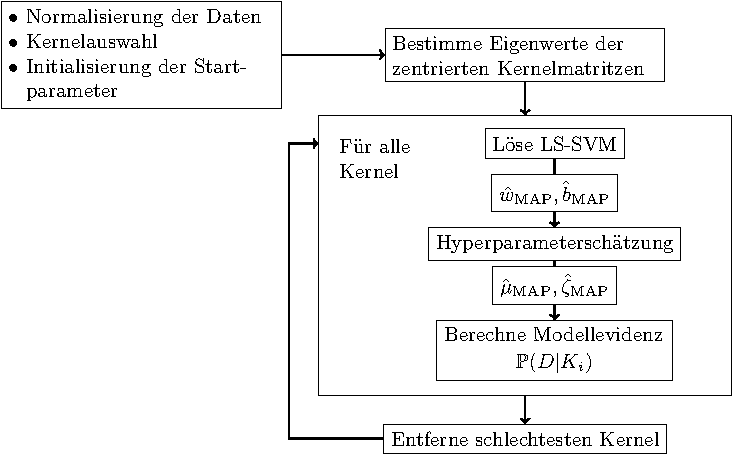
\includegraphics[scale=0.9]{Algo.pdf}
\end{frame}

\begin{frame}
	\centering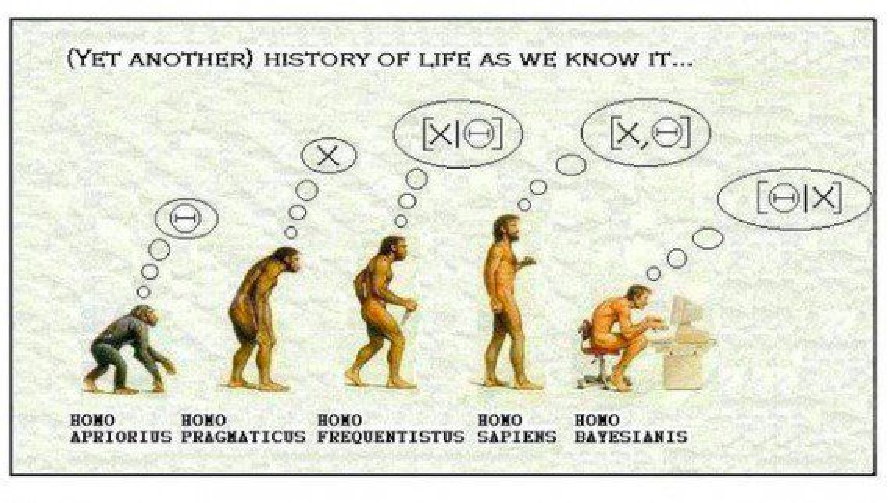
\includegraphics[scale=0.7]{humanshistory.pdf}
\end{frame}


%KICK ME?



%dann beispiel, curse of dimensionality, bezug zu networks, variational techniques
%hierarchical modelling evtl! (bei nets mit autoerkennung und marken mega coole anwendung!


\begin{frame}{Quellen und weiterführende Literatur}
	\begin{itemize}
	
	\item Aki Vehtari, Janne Ojanen; A survey of Bayesian predictive 						  methods for model assessment, selection and comparison; Statistics 				  Surveys; Vol. 6 142-228; 2012
	\item T. Van Gestel et. al.; Bayesian Framework for Least-Squares Support 				  Vector Machine Classifiers, Gaussian Processes, and Kernel Fisher
		  Discriminant Analysis; Neural Computation 14, 1115–1147; 2002
	\end{itemize}
\end{frame}


\end{document}